\chapter{Results and Discussion}
\label{chapter:results}
In this section, we present the attempts made to achieve the best outcome along with the respective intermediate results obtained at various steps.
We discuss the outcomes of the best approach, as described in Chapter \ref{chapter:methodology}, and the enhanced visualization of skeletal clusters. The originally planned work underwent modifications due to constraints posed by a limited and imbalanced dataset. Additionally, challenges were encountered in sourcing additional complete and consistent samples to augment the dataset.

Subsequent sections offer a summary of the accomplished results and potential implications. The focus lies on performance analysis concerning operational conditions and proposes future developments aimed at enhancing the obtained results.
\section{Graph-based Framework}
The OoM was classified using three distinct features: velocity, acceleration and angular momentum, as described in Section \ref{subsec:alg_features}.
For each feature, we applied two different similarity functions, as part of the pipeline explained in Chapter \ref{sec:graph_method}.
The two similarity functions are the \textit{Cosine Similarity} (concept explained in Section \ref{sec:cosine_sim}) and a custom function described in Section \ref{sec:starting_point}.

In Table \ref{tab:clust_results} we can see that the Cosine similarity outperforms the custom-made function. 
Therefore, it was chosen as the similarity function for this specific dataset.

\begin{table}[H]
  \centering
  \begin{tabular}{||>{\centering\arraybackslash}p{4.3cm}||>{\centering\arraybackslash}p{2.0cm}||>{\centering\arraybackslash}p{2.7cm}||>{\centering\arraybackslash}p{4.4cm}||}
  \hline
  \textbf{Similarity Function} & \textbf{Speed} & \textbf{Acceleration} & \textbf{Angular Momentum} \\
  \hline
  Cosine & 28.3\%  & 26.7\%  & 36.6\%  \\
  \hline
  Custom & 18\%  & 21.1\%  & 34.2\%  \\
  \hline
  \end{tabular}
  \caption{Classification accuracy over the whole dataset obtained by using the two different similarity functions}
  \label{tab:clust_results}
\end{table}

From here on, the graphs will reflect the results obtained using cosine similarity as the measurement method.
While these results may not be exceptional, they still outperform a random approach, in which two random nodes are selected and compared to the ground truth. \\
Infact such an approach, achieves an accuracy of 19.4\% 
The formula to calculate the probability of picking at least one joint of the two is shown in Equation \ref{eq:prob_rand}
\begin{equation}
  \mathbb{P}(\textit{picking at least one of the two joints}) = \frac{\binom{2}{1} \binom{18}{1}}{\binom{20}{2}} + \frac{\binom{2}{2} \binom{18}{0}}{\binom{20}{2}} = \frac{37}{190} \cong 19.4 \%
  \label{eq:prob_rand}
\end{equation}
  
%TODO controllare probabilità

In Figure \ref{fig:wdc_results} we can see the distribution of the results for each edge of the dataset with respecto to their ground truth.
The WDC method seems to perform reasonably well in classifying sources of movement in the upper part of the body, where there are generally a greater number of edges per node.
But performs generally bad on lower body and the most borderline nodes (those connected to the rest of the graph by only one arc).\\
This might suggest that by varying the number of clusters to allow for the creation of smaller clusters, perhaps using a hierarchical clustering approach, it could be possible to isolate multiple splits of the same body part.\\ 
However, it is essential to take these results with caution because the dataset is very small and certainly does not have a statistically significant sample of each class. 
Nevertheless, it remains a good starting point. \\

\begin{figure}[H]
  \centering
  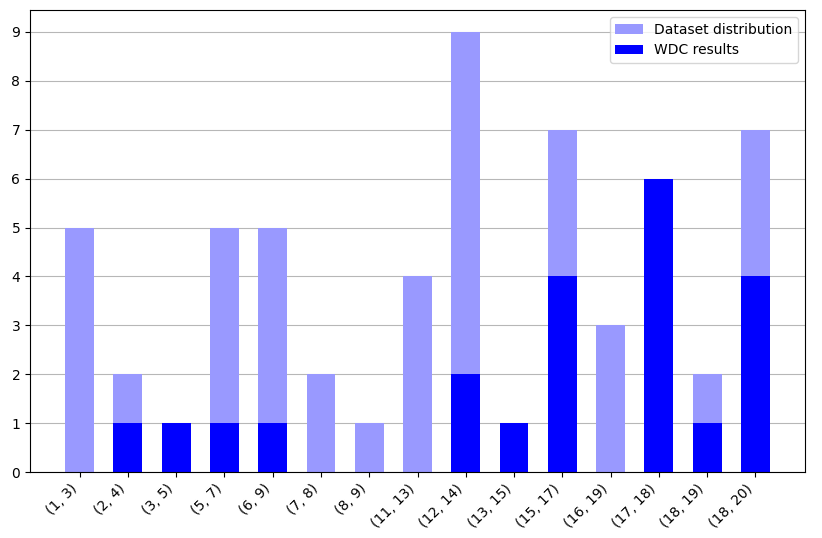
\includegraphics[width=0.85\textwidth]{wdc_results.png}
  \caption{Joints and frequency of the dataset and the correctly classified graph-based algorithm applied on the angular momentum feature}
  \label{fig:wdc_results}
\end{figure}

\section{Clusters Stabilization}
In this first example, in Figure \ref{fig:stabilization_results}, we can observe the results of stabilization of three clusters with the same color scheme applied on two different time instants. 
In (a), the preceding time instant is visible, while (b) showcases the subsequent time instant in an unstabilized state. 
In (c) instead, the subsequent time instant with clusters stabilized.
\begin{figure}[H]
  \centering
  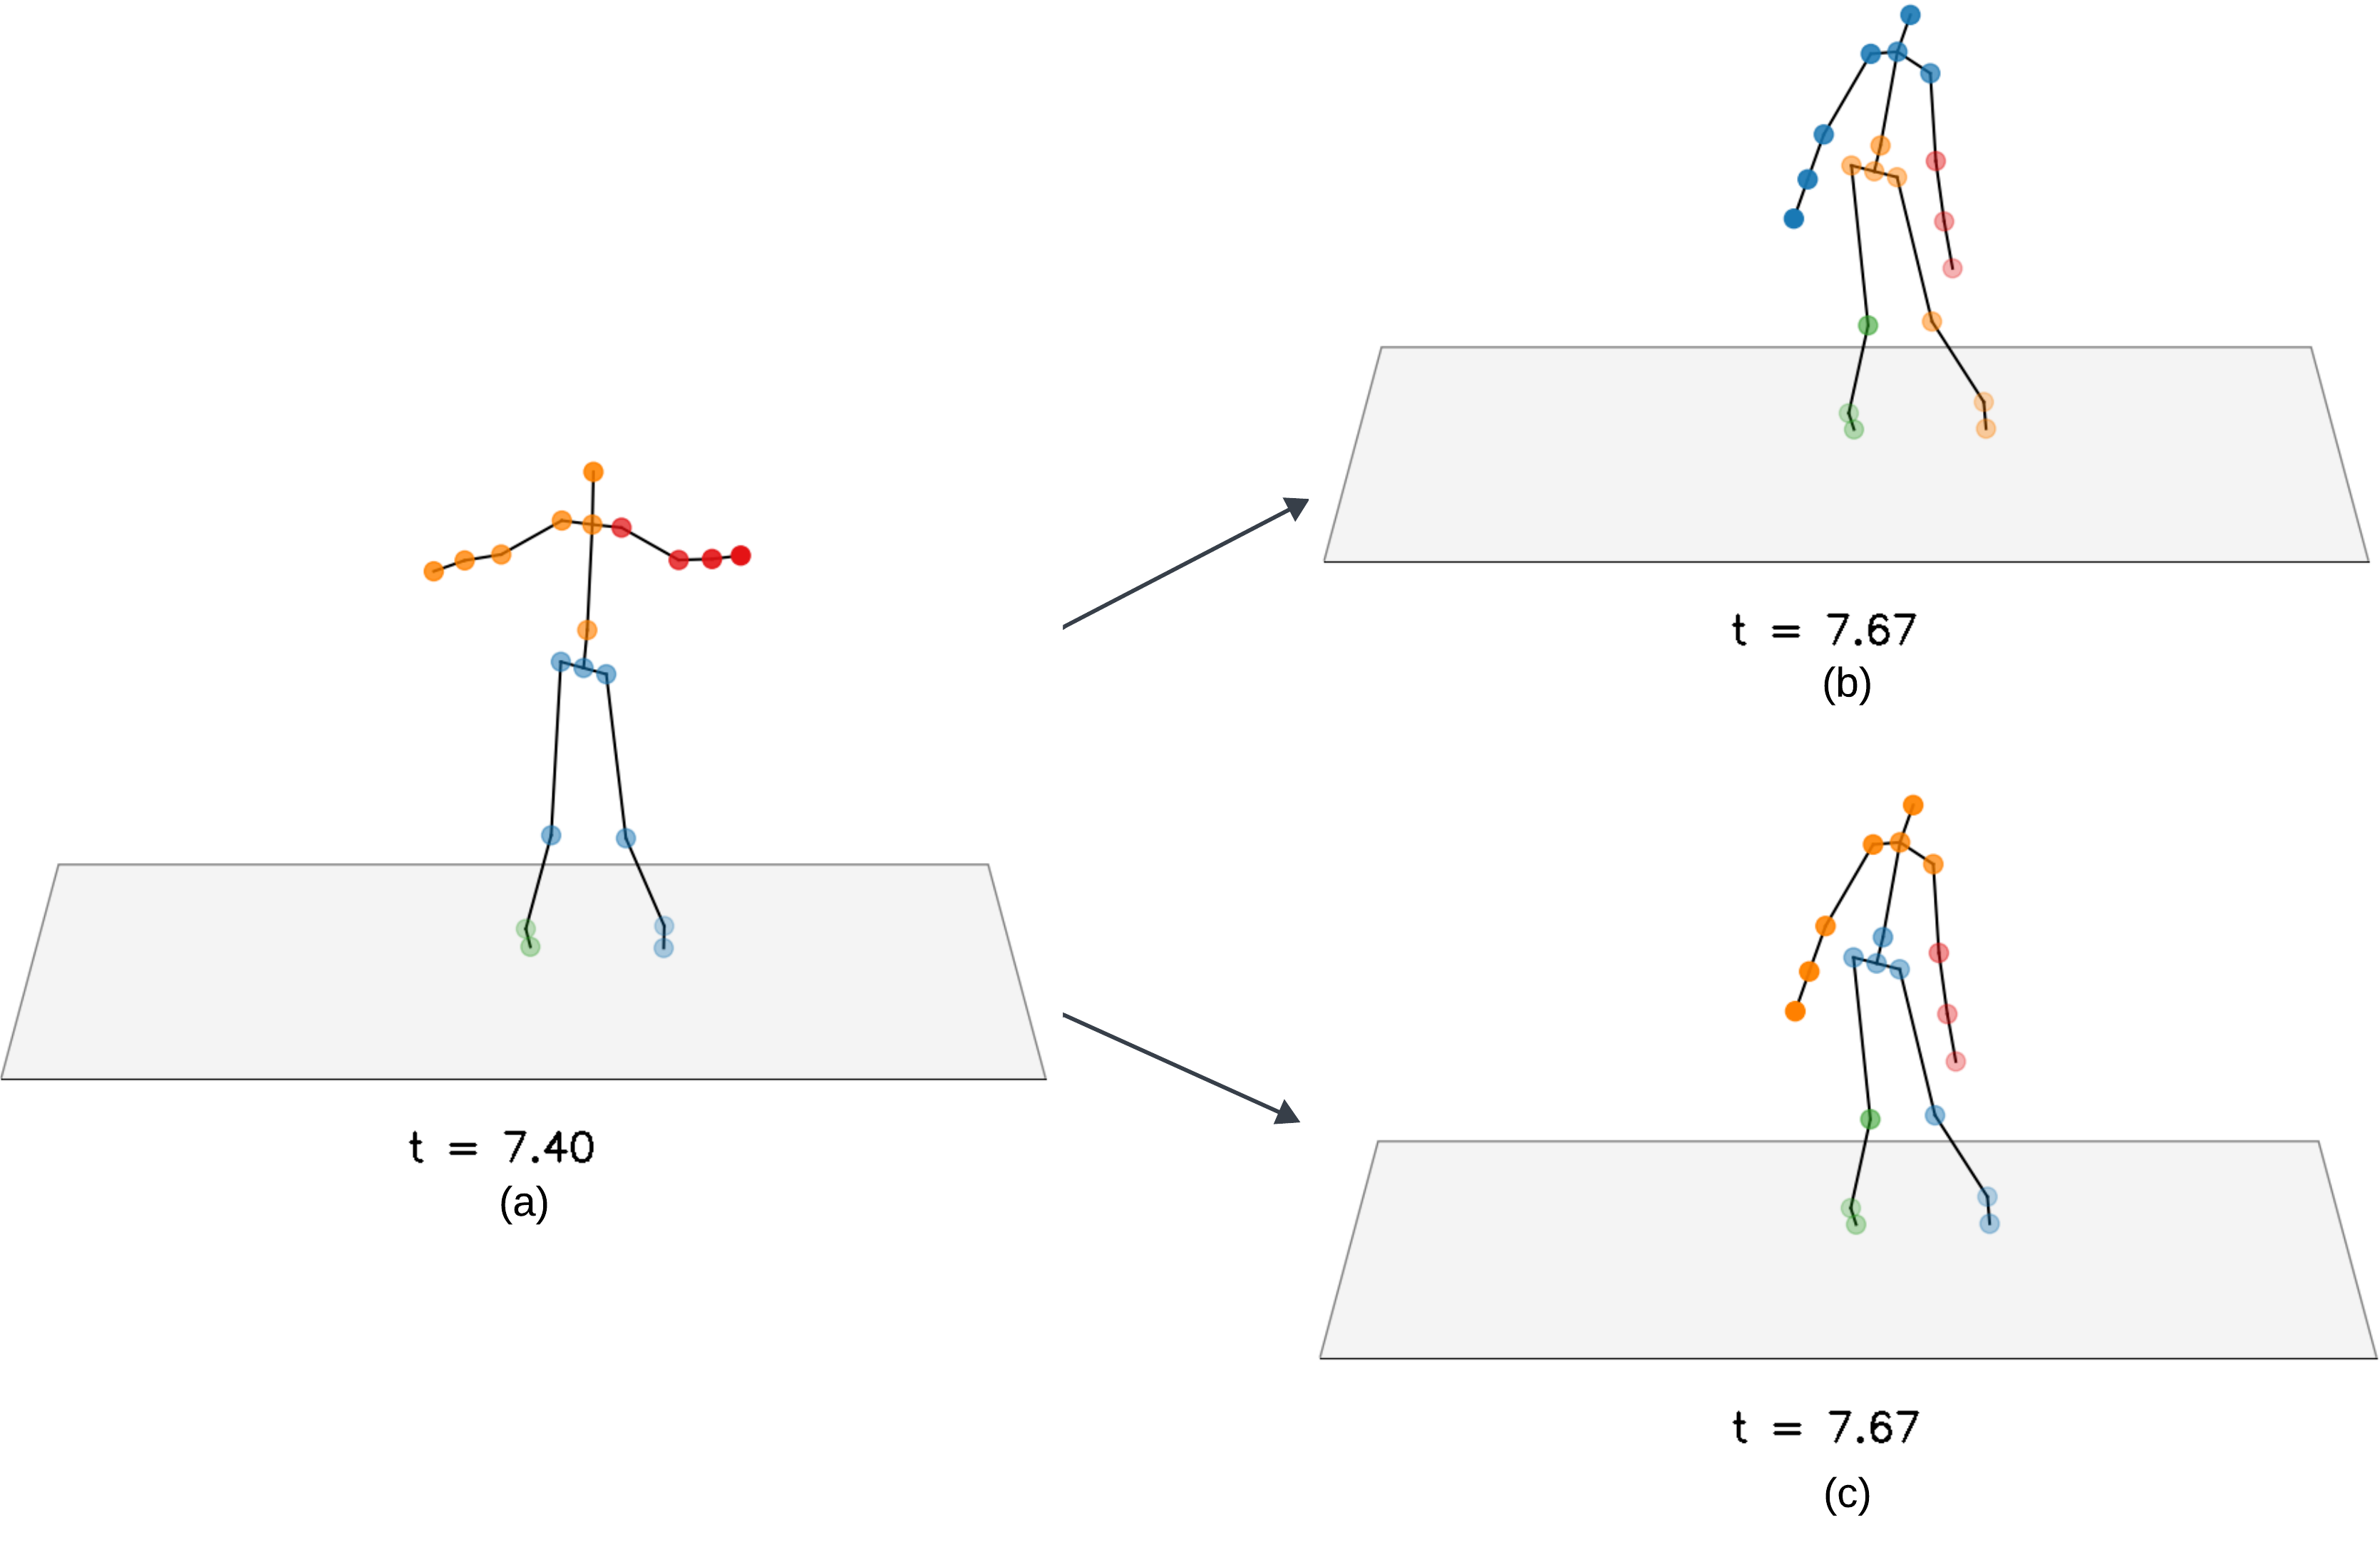
\includegraphics[width=0.9\textwidth]{ClustersStabilization.png}
  \caption{Clustering at $t=7.40$ (a), $t=7.67$ unstabilized (b), and $t=7.67$ stabilized (c).}
  \label{fig:stabilization_results}
\end{figure}

A further extension of this concept for visualization purposes can be applied by analyzing a movement evolving in realtime, by recording a small segment of video, which is able to provide a better view of the stabilization outcomes.
The transition smoothing algorithm explained in Section \ref{subsec:clusters_smoothing} is here visualized in the videos whose link has been embedded in the QR code in Figure \ref{fig:qr_movements}. \\

These 3 QR codes lead to a video that represents the same movement in the 20 joints skeleton, where the dancer begins from a stance with slightly spread legs and the left arm raised upwards.
Throughout the movement, the left arm descends while moving backward, the torso leans forward, taking the right arm along with it, and the left foot lifts off the ground, walking back to follow the left arm.\\

The first QR (Figure \ref{fig:qr_movement_pure}) leads to the original clustering method without the application of any stabilization method, visually it can be clearly seen how the instability of the simple clustering creates a flickering effect, resulting in a poor visualization capability.
Instead the second (Figure \ref{fig:qr_movement_stabilized}), which is the stabilized version the flickering has been removed by swapping the clusters colors on subsequent frames based on the proposed approach mentioned in Section \ref{subsec:clustering_stabilization}.
Moreover by applying this method the recognition of eventual origins of movement where they can be clearly seen in a video segment is facilitated. \\

In the last one (Figure \ref{fig:qr_movement_smooth}), clusters' evolution is further smoothed by picking the node with highest degree centrality of the cluster every 5 frames in a 100 fps video.
By further smoothing the clusters transition one can also visually inspect the appearing of multiple origins at the expense of the continuity of each cluster. 
Infact with this method the clusters will have transitory frames in which are inconsistent.

\begin{figure}[H]
  \centering
  \begin{subfigure}[b]{0.49\textwidth}
    \centering
    
\includegraphics[width=\textwidth]{qrcode_clustering_pure.png}
    \caption{}
    \label{fig:qr_movement_pure}
  \end{subfigure}
  \hfill
  \begin{subfigure}[b]{0.49\textwidth}
    \centering
    
\includegraphics[width=\textwidth]{qrcode_clustering_stabilized.png}
    \caption{}
    \label{fig:qr_movement_stabilized}
  \end{subfigure}
  \hfill
  \begin{subfigure}[b]{0.49\textwidth}
    \centering
    
\includegraphics[width=\textwidth]{qrcode_clustering_smooth.png}
    \caption{}
    \label{fig:qr_movement_smooth}
  \end{subfigure}
  \caption{QR codes referencing to the pure clustering method (a), the stabilized version (b) and a combination of stabilization and smoothing (c)}
  \label{fig:qr_movements}
\end{figure}
\clearpage

In conclusion, the MaxWPM algorithm is able to provide a clearer and more consistent visualization of clusters, allowing us to understand which joints are most similar during motion, without abrupt color changes. \\
Furthermore, the additional smoothing technique allows to better see the evolution of clusters across a longer timespan also in those cases where in a short amount of time clusters still tend to change too fast.\\



\clearpage

\section{Machine Learning}

\paragraph{Prior Attempts}
The refinement process of the results went through various attempts, as illustrated here. 
We began with the RF as the initial model, suggested as the best option in previous works in the field of motion analysis \cite{oneto:2020}, with a hyperparameter $n\_estimators = 400$, a generally sufficient value.

The tests to identify the best model were performed on the most frequent edge of the dataset, \textit{left\_hand - left\_wrist}, aiming to balance TPR and TNR.

We directly started with LOOCV as the validation strategy, attempting to rebalance the dataset by applying various balancing strategies. 
Initially, we attempted a strategy using the \textit{Random Undersampler}, a classic sampling method where the majority class is reduced by randomly extracting the same number of samples as the minority class. 
These samples were then used for balanced training.

The initial results were quite promising, as depicted in the confusion matrix shown in Table \ref{tab:ml_results_cm_trial1}. 
However, we decided to discard the undersampling approach, considering that with an already limited number of diverse movements, further reducing the number of samples would lead to significant information loss. 
This conclusion is also supported by the relatively high FP rates, indicating that the model tends to classify a sample as positive with too much confidence.
\begin{table}[H]
  \centering
  \renewcommand{\arraystretch}{1.5} % Aumenta lo spazio tra le righe del doppio
  \begin{tabular}{|>{\centering\arraybackslash}p{0.5cm}|>{\centering\arraybackslash}p{0.5cm}|}
  \hline
  41 & 10 \\
  \hline
  2 & 7 \\
  \hline
  \end{tabular}
  \caption{Confusion matrix for Random Undersampler and LOOCV strategy}
  \label{tab:ml_results_cm_trial1}
\end{table}

Even applying a \textit{Random Oversampling} strategy to the minority class (while still excluding the testing sample for each iteration of LOOCV) yields poor results, as seen in Table \ref{tab:ml_results_cm_trial2}.
\begin{table}[H]
  \centering
  \renewcommand{\arraystretch}{1.5} % Aumenta lo spazio tra le righe del doppio
  \begin{tabular}{|>{\centering\arraybackslash}p{0.5cm}|>{\centering\arraybackslash}p{0.5cm}|}
  \hline
  51 & 0 \\
  \hline
  8 & 1 \\
  \hline
  \end{tabular}
  \caption{Confusion matrix for Random Oversampler and LOOCV strategy}
  \label{tab:ml_results_cm_trial2}
\end{table}
We realized during the various trials that to achieve better results, we needed to carefully choose the resampling strategy. 
Therefore, we explored alternatives capable of artificially creating samples to better represent the boundaries in the multidimensional space of our features, rather than emphasizing individual points.

Among these alternatives, we also experimented with the SMOTE algorithm, which generates synthetic data by uniformly interpolating points in the multidimensional feature space, and ADASYN, which serves the same purpose as SMOTE but estimates data distribution for resampling.

Below, in Table \ref{tab:ml_results_cm_trial3} and \ref{tab:ml_results_cm_trial4}, the confusion matrices for the two algorithms are presented.
\begin{figure}[H]
  \centering
  \begin{subfigure}{0.4\textwidth}
    \centering
    \renewcommand{\arraystretch}{1.5} % Increase row spacing by double
    \begin{tabular}{|>{\centering\arraybackslash}p{0.5cm}|>{\centering\arraybackslash}p{0.5cm}|}
      \hline
      50 & 1 \\
      \hline
      6 & 3 \\
      \hline
    \end{tabular}
    \caption{}
    \label{tab:ml_results_cm_trial3}
  \end{subfigure}
  \hspace{1cm} % Horizontal space between the two tables
  \begin{subfigure}{0.4\textwidth}
    \centering
    \renewcommand{\arraystretch}{1.5} % Increase row spacing by double
    \begin{tabular}{|>{\centering\arraybackslash}p{0.5cm}|>{\centering\arraybackslash}p{0.5cm}|}
      \hline
      51 & 0 \\
      \hline
      5 & 4 \\
      \hline
    \end{tabular}
    \caption{}
    \label{tab:ml_results_cm_trial4}
  \end{subfigure}
  \caption{Confusion matrices of the SMOTE and ADASYN algorithms}
\end{figure}

In general, these methods exhibit promising results with almost no parameterization required. 
However, a notable observation is that while the \textit{Random Undersampler} demonstrates similar and high TPR and TNR, it might be challenging to improve significantly due to its simplicity. 
The same notion applies to the \textit{Random Oversampler}.

Regarding SMOTE and ADASYN, they compete with each other, but ADASYN remains challenging to apply because of its reduced number of samples, making it difficult to infer from such a limited data distribution.
In Table \ref{tab:ml_trials_metrics}

\begin{table}[H]
  \centering
  \begin{tabular}{||>{\centering\arraybackslash}p{5.0cm}||>{\centering\arraybackslash}p{1.5cm}||>{\centering\arraybackslash}p{1.5cm}||>{\centering\arraybackslash}p{1.5cm}||>{\centering\arraybackslash}p{2.5cm}||}
  \hline
  \textbf{Method} & \textbf{TPR} & \textbf{TSS} &\textbf{TNR} &\textbf{Accuracy}\\
  \hline
  Random Undersampler & 78\% & 79\% & 80\% & 82\%  \\
  \hline
  Random Oversampler & 11\% & 56\% & 100\% & 87\%  \\
  \hline
  SMOTE & 33\% & 66\% & 98\% & 88\%  \\
  \hline
  ADASYN & 44\% & 72\% & 100\% & 92\%  \\
  \hline
  \end{tabular}
  \caption{Metrics of different methods on the most frequent class of the dataset}
  \label{tab:ml_trials_metrics}
\end{table}

Finally, considered the potential presence of zones with single points that might have been marginalized during the minimization phase of the Gini impurity loss function and others that could be more dense, which means that are been sufficiently represented, we opted for a variation of the SMOTE.\\
This assumpution lead us to the B-SMOTE to have a better representativeness of those marginalized samples. 
By balancing the two characteristic hyperparameters of B-SMOTE (\textit{k\_neighbors} and \textit{m\_neighbors}) in proportion to the ratio between the sizes of the two classes, we aimed to refine the model.

The final result was based on expanding the minority class, training a RF with numerous trees to thoroughly comprehend the best features to select, and subsequently reducing the learning of a second forest optimized on a smaller subset of features.





\paragraph{Best Results}
In the following Tables (from \ref{tab:ml_results_cm_joints} to \ref{tab:ml_results_cm_body_parts}), there are the confusion matrices, the TPR, TSS, TNR and the Accuracy score for the final model defined in Section \ref{sec:ml_method} in our three formulations:
\begin{itemize}
  \item The most frequent 6 classes of our dataset (Table \ref{tab:ml_results_cm_joints} and \ref{tab:ml_results_joints}) in the by-joint-subdivision.
  \item The 5 boby parts in which have been grouped the joints (Table \ref{tab:ml_results_cm_body_parts} and \ref{tab:ml_results_body_parts})
  \item The division into the upper and lower body part, which is in the same tables.
\end{itemize} 
To interpret the meaning of the confusion matrices, please refer to Section \ref{subsec:evaluation_metrics}.
This is because the dataset is unbalanced, and therefore, better prediction results are expected from this class.
As observed, accuracy consistently remains very high, almost always exceeding 70\%.
However, beyond this, the model demonstrates high $specificity$, meaning it excels at maximizing TN but struggles to identify TP effectively.
This behavior is evident in the TPR, which varies significantly across different classes.
The model requires a high level of certainty in predictions before classifying a sample as positive.
You can also observe the model's high specificity from the TNR, which is consistently quite high in all cases, typically greater than 80\%. \\

Furthermore, for a more comprehensive assessment of the results, we included the TSS, normalized between 0 and 1 and presented as a percentage. 
This metric is considered effective in demonstrating the model's potential to balance predictions and overall incorrect predictions.

As the TSS ranges from -1 (performing poorly in both cases), 0 (performing well in one case but poorly in the other), to 1 (performing well in both cases), in our case, after shifting and scaling, 
we observed the TSS consistently exceeding halfway, signifying that the model is generally successful in minimizing errors across all predictions. 

\clearpage
\begin{table}[H]
    \centering
    \renewcommand{\arraystretch}{1.5} % Aumenta lo spazio tra le righe del doppio
    \begin{subfigure}[b]{0.1\textwidth}
        \centering
        \begin{tabular}{|>{\centering\arraybackslash}p{0.5cm}|>{\centering\arraybackslash}p{0.5cm}|}
        \hline
        48 & 3 \\
        \hline
        3 & 6 \\
        \hline
        \end{tabular}
        \caption{}
        \label{tab:ml_results_cm_edge_1}
    \end{subfigure}
    \hspace{0.05\linewidth}
    \begin{subfigure}[b]{0.1\textwidth}
        \centering
        \begin{tabular}{|>{\centering\arraybackslash}p{0.5cm}|>{\centering\arraybackslash}p{0.5cm}|}
        \hline
        51 & 2 \\
        \hline
        6 & 1 \\
        \hline
        \end{tabular}
        \caption{}
        \label{tab:ml_results_cm_edge_2}
    \end{subfigure}
    \hspace{0.05\linewidth}
    \begin{subfigure}[b]{0.1\textwidth}
        \centering
        \begin{tabular}{|>{\centering\arraybackslash}p{0.5cm}|>{\centering\arraybackslash}p{0.5cm}|}
        \hline
        44 & 9 \\
        \hline
        7 & 0 \\
        \hline
        \end{tabular}
        \caption{}
        \label{tab:ml_results_cm_edge_3}
    \end{subfigure}
    \hspace{0.05\linewidth}
    \begin{subfigure}[b]{0.1\textwidth}
        \centering
        \begin{tabular}{|>{\centering\arraybackslash}p{0.5cm}|>{\centering\arraybackslash}p{0.5cm}|}
        \hline
        51 & 3 \\
        \hline
        4 & 2\\
        \hline
        \end{tabular}
        \caption{}
        \label{tab:ml_results_cm_edge_4}
    \end{subfigure}
    \hspace{0.05\linewidth}
    \begin{subfigure}[b]{0.1\textwidth}
        \centering
        \begin{tabular}{|>{\centering\arraybackslash}p{0.5cm}|>{\centering\arraybackslash}p{0.5cm}|}
        \hline
        52 & 3 \\
        \hline
        4 & 1 \\
        \hline
        \end{tabular}
        \caption{}
        \label{tab:ml_results_cm_edge_5}
    \end{subfigure}
    \hspace{0.05\linewidth}
    \begin{subfigure}[b]{0.1\textwidth}
        \centering
        \begin{tabular}{|>{\centering\arraybackslash}p{0.5cm}|>{\centering\arraybackslash}p{0.5cm}|}
        \hline
        53 & 2 \\
        \hline
        2 & 3 \\
        \hline
        \end{tabular}
        \caption{}
        \label{tab:ml_results_cm_edge_6}
    \end{subfigure}
    \caption{Confusion matrices of the 6 most frequent classes in the dataset}
    \label{tab:ml_results_cm_joints}
\end{table}


\begin{table}[H]
    \centering
    \begin{tabular}{||>{\centering\arraybackslash}p{1.2cm}||>{\centering\arraybackslash}p{5.7cm}||>{\centering\arraybackslash}p{1.3cm}||>{\centering\arraybackslash}p{1.2cm}||>{\centering\arraybackslash}p{1.3cm}||>{\centering\arraybackslash}p{1.9cm}||}
    \hline
    \textbf{Label} & \textbf{Edge} & \textbf{TPR} & \textbf{TSS} &\textbf{TNR} &\textbf{Accuracy}\\
    \hline
    (a) & left\_hand - left\_wrist  & 66\% & 80\% & 94\% & 90\%  \\
    \hline
    (b) & shoulder\_center - head  & 14\% & 55\% & 96\% & 87\% \\
    \hline
    (c) & right\_elbow - right\_shoulder  & 0\%  & 42\% & 83\% & 73\% \\ 
    \hline
    (d) & right\_shoulder - shoulder\_center & 33\% & 64\% & 94\% & 88\%\\
    \hline
    (e) & right\_knee - right\_hip  & 20\% & 57\% & 95\% & 88\%  \\
    \hline
    (f) & left\_knee - left\_hip  & 60\% & 78\% & 96\% & 93\% \\ 
    \hline
    \end{tabular}
    \caption{Metrics of the 6 classes most frequent of the dataset}
    \label{tab:ml_results_joints}
\end{table}




\begin{table}[H]
  \centering
  \begin{subfigure}[b]{0.1\textwidth}
    \centering
    \renewcommand{\arraystretch}{1.5} % Aumenta lo spazio tra le righe del doppio
    \begin{tabular}{|>{\centering\arraybackslash}p{0.5cm}|>{\centering\arraybackslash}p{0.5cm}|}
    \hline
    37 & 5 \\
    \hline
    7 & 11 \\
    \hline
    \end{tabular}
    \caption*{\textbf{(g)}}
    \label{tab:ml_results_cm_body_part_1}
  \end{subfigure}
  \hspace{0.05\linewidth}
  \begin{subfigure}[b]{0.1\textwidth}
    \centering
    \begin{tabular}{|>{\centering\arraybackslash}p{0.5cm}|>{\centering\arraybackslash}p{0.5cm}|}
    \hline
    37 & 9 \\
    \hline
    10 & 4 \\
    \hline
    \end{tabular}
    \caption*{\textbf{(h)}}
    \label{tab:ml_results_cm_body_part_2}
  \end{subfigure}
  \hspace{0.05\linewidth}
  \begin{subfigure}[b]{0.1\textwidth}
    \centering
    \begin{tabular}{|>{\centering\arraybackslash}p{0.5cm}|>{\centering\arraybackslash}p{0.5cm}|}
    \hline
    43 & 4 \\
    \hline
    6 & 7 \\
    \hline
    \end{tabular}
    \caption*{\textbf{(i)}}
    \label{tab:ml_results_cm_body_part_3}
  \end{subfigure}
  \hspace{0.05\linewidth}
  \begin{subfigure}[b]{0.1\textwidth}
    \centering
    \begin{tabular}{|>{\centering\arraybackslash}p{0.5cm}|>{\centering\arraybackslash}p{0.5cm}|}
    \hline
    47 & 5 \\
    \hline
    7 & 1\\
    \hline
    \end{tabular}
    \caption*{\textbf{(l)}}
    \label{tab:ml_results_cm_body_part_4}
  \end{subfigure}
  \hspace{0.05\linewidth}
  \begin{subfigure}[b]{0.1\textwidth}
    \centering
    \begin{tabular}{|>{\centering\arraybackslash}p{0.5cm}|>{\centering\arraybackslash}p{0.5cm}|}
    \hline
    51 & 2 \\
    \hline
    6 & 1 \\
    \hline
    \end{tabular}
    \caption*{\textbf{(m)}}
    \label{tab:ml_results_cm_body_part_5}
  \end{subfigure}
  \hspace{0.05\linewidth}
  \begin{subfigure}[b]{0.1\textwidth}
    \centering
    \begin{tabular}{|>{\centering\arraybackslash}p{0.5cm}|>{\centering\arraybackslash}p{0.5cm}|}
        \hline
        16 & 5 \\
        \hline
        8 & 31 \\
        \hline
    \end{tabular}
    \caption*{\textbf{(n)}}
    \label{tab:ml_results_cm_body_part_6}
  \end{subfigure}
  \caption{Confusion matrices of the 5 Body Parts and of the Upper/Lower part}
  \label{tab:ml_results_cm_body_parts}
\end{table}


\begin{table}[H]
    \centering
    \begin{tabular}{||>{\centering\arraybackslash}p{1.2cm}||>{\centering\arraybackslash}p{5.7cm}||>{\centering\arraybackslash}p{1.3cm}||>{\centering\arraybackslash}p{1.2cm}||>{\centering\arraybackslash}p{1.3cm}||>{\centering\arraybackslash}p{1.9cm}||}
        \hline
        \textbf{Label} & \textbf{Body Part} & \textbf{TPR} & \textbf{TSS} & \textbf{TNR} & \textbf{Accuracy} \\
        \hline
        (g) & Right Arm  & 61\% & 75\% & 88\% & 80\%  \\
        \hline
        (h) & Left Arm & 29\% & 55\% & 80\% & 68\% \\
        \hline
        (i) & Right Leg  & 54\% & 73\% & 91\% & 83\% \\ 
        \hline
        (l) & Left Leg & 12\% & 51\% & 90\% & 80\%  \\
        \hline
        (m) & Head  & 14\% & 55\% & 96\% & 86\% \\
        \hline
        \hline
    \end{tabular}
    \begin{tabular}{||>{\centering\arraybackslash}p{1.2cm}||>{\centering\arraybackslash}p{5.7cm}||>{\centering\arraybackslash}p{1.3cm}||>{\centering\arraybackslash}p{1.2cm}||>{\centering\arraybackslash}p{1.3cm}||>{\centering\arraybackslash}p{1.9cm}||}
        \textbf{Label} & \textbf{Body Part} & \textbf{TPR} & \textbf{TSS} & \textbf{TNR} & \textbf{Accuracy} \\
        \hline
        (n) & Upper & 79\% & 78\% & 76\% & 78\% \\
        \hline
    \end{tabular}
    \caption{Metrics of the 5 Body Parts and the Upper}
    \label{tab:ml_results_body_parts}
\end{table}

From the results obtained in Table \ref{tab:ml_results_joints}, a fluctuating trend is evident, probably due to the limited and imbalanced data. 
Despite efforts to balance the dataset, as they were tested solely on the majority class among the available ones, whose results can be seen in the confusion matrix in Table \ref{tab:ml_results_cm_edge_1}, 
they were not sufficient to compensate for the lack of data in the other classes. \\
What has been achieved, therefore, is an effectiveness in predicting the majority class effectively and a tendency to balance FN and FP. 
By merging the classes, as done in Q2 and Q3, the fluctuations in the results appear to be somewhat mitigated at the expense of a slight deterioration in overall performance (Table \ref{tab:ml_results_body_parts}).
With an extension of the dataset, better and more robust accuracies can be achieved across all classes.
Furthermore, it would also be possible to perform multiclass classification for recognition of multiple origin of movements from the same movement.\\

Further insights of the model can be infered by looking at the ROC curve and it's corresponding AUC, in particular let's see what the one associated to the most frequent joint tells us (Figure \ref{fig:roc_auc_results}):
By following the thresholds we can see that $Thresh = 0.28$ provides the best results. This means that by thresholding in that way the output of the forest (which is a score) we can achieve a 90\% of TPR with just a 20\% of FPR.
By default the RF will apply a threshold of $0.5$ (in other words classify as positive a sample whose score is greater than $0.5$).\\

Moreover, with an AUC of $0.83$, it's evident that the model has almost reached curve saturation. This signifies the model's high performance level.

\begin{figure}[H]
  \centering
  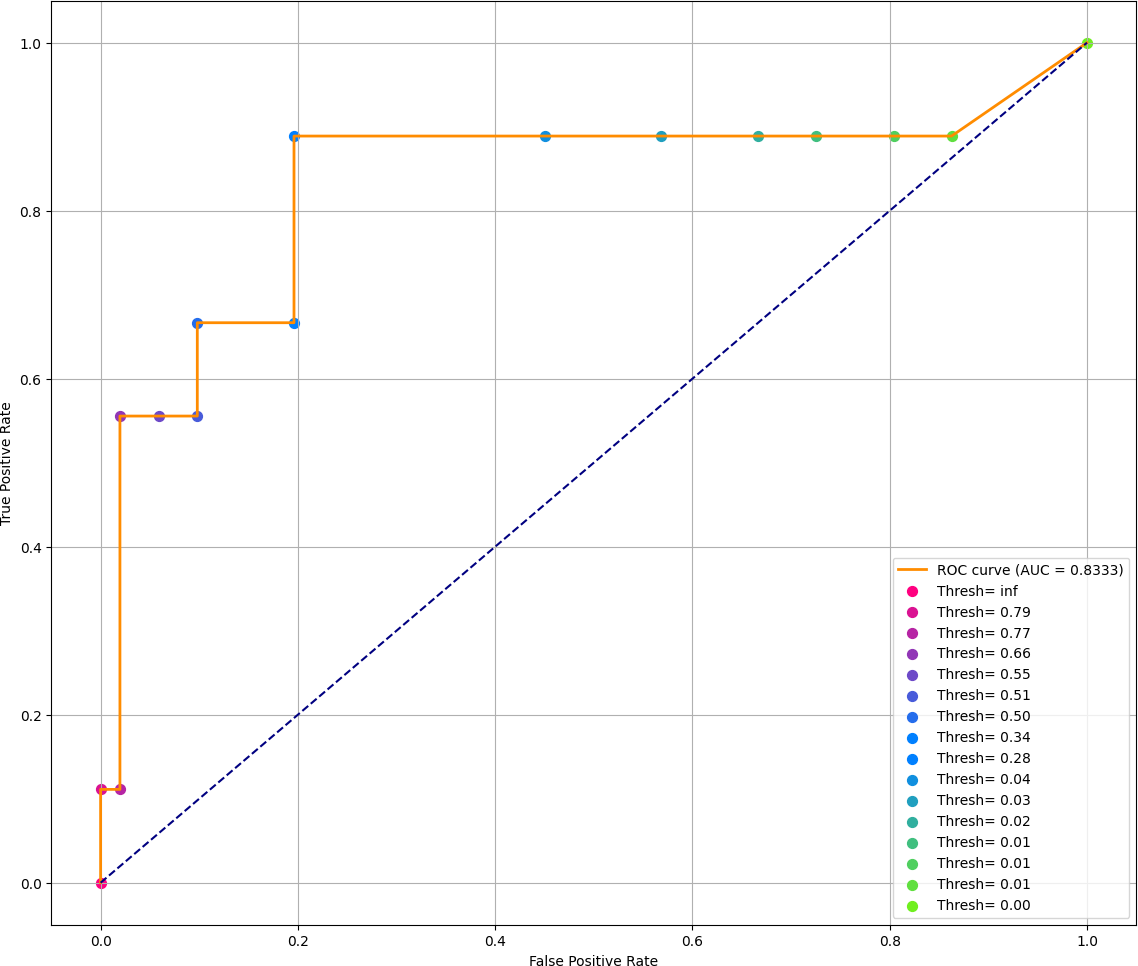
\includegraphics[width=0.66\textwidth]{ROC_AUC_result_best_joint.png}
  \caption{ROC curve of the most frequent joint of the dataset}
  \label{fig:roc_auc_results}
\end{figure}

Moreover, it is essential to note that the results remained unstable, and the previous ones were the best outcomes across multiple runs of the algorithm, as explained in Section \ref{subsec:loocv_theoretical} of the LOOCV.\\
To compensate for this, 30 runs were executed, and the mean and variance of the main metrics were calculated.
In Table \ref{tab:overall_results}, it can be observed that the metrics on the majority class remain generally high, but with a variability that exceeds 10\% in terms of standard deviation.
Meanwhile, the minority class presents intermediate scores, as expected from the model.\\
Finally, concerning the overall accuracy, it also averages at 0.868 with a standard deviation of 0.023.

\begin{table}[H]
  \centering
  \begin{tabular}{||>{\centering\arraybackslash}p{1.8cm}||>{\centering\arraybackslash}p{1.9cm}||>{\centering\arraybackslash}p{1.9cm}||>{\centering\arraybackslash}p{1.3cm}||>{\centering\arraybackslash}p{1.3cm}||>{\centering\arraybackslash}p{1.7cm}||>{\centering\arraybackslash}p{1.7cm}||}
  \hline
  \textbf{Class} & \textbf{precision mean} & \textbf{precision std} & \textbf{recall mean} &\textbf{recall std} &\textbf{f1-score mean} &\textbf{f1-score std} \\
  \hline
  Negative & 0.934 & 0.010 & 0.909 & 0.025 & 0.921 & 0.015 \\
  \hline
  Positive & 0.560 & 0.077 & 0.637 & 0.058 & 0.594 & 0.057 \\
  \hline
  \end{tabular}
  \caption{Statistics of the metrics for the most frequent joint binary classification}
  \label{tab:overall_results}
\end{table}

\clearpage


\section{Future researches}
\label{sec:future_researches}
There are several possible future extensions of this work, that could improve on the method and yield better results. \\

To improve prediction accuracy, we aim to expand the dataset and ensure balance by incorporating new, intentionally designed movement segments.
This will be done without introducing overly intricate motions that could potentially complicate the movement classification.\\

In future revisions, with a more extensive dataset, additive methods could be employed to measure the amount of useful information added by the WDC approach in a classification problem compared to the other high-level features used.
To move towards real-time automatic classification, markerless MoCap can be useful.\\

Achieving real-time classification with a marker-based system is highly improbable.
Although markerless systems may exhibit lower precision in comparison to marker-based systems, 
they represent a viable alternative for real-world applications.\\

Another potential future expansion of this concept could involve a study on movement fragments characterized by multiple origins.
This would be valuable in examining, for instance, during the act of catching a ball, whether the movement origin is symmetrically distributed throughout the body or if there is a dominant component compared to the others.\\

The final extension of our thesis involves the examination of small groups of individuals and the exploration of how coordinated movement patterns emerge within these groups.
Instead of treating individual joints as players, it can be adopted a similar approach within the framework of graph and game theory, but at a higher anatomical level.
Here, the group of individuals operates as a cohesive unit, where each person in the group takes on the role of a player. 
This approach enables to examine leading behaviors, including those exhibited by individual initiators whose movements influence the entire group.
In scenarios with a limited number of potential permutations for clustering, the advantages between favoring the Hungarian algorithm or the BF approach are not substantial. 
However, in more intricate situations involving numerous nodes, such as those with groups of people, selecting the most efficient algorithm for graph manipulation becomes crucial to achieve real-time feasibility.
